\chapter{Appendix}
\label{ch:appendix}
The appendix contains the schematic of the two boards that were created for the prototype. 

\section{Schematic of PCB and FlexPCB}
\label{ch:appendix:pcb_flexpcb}

\begin{figure}
    \centering
    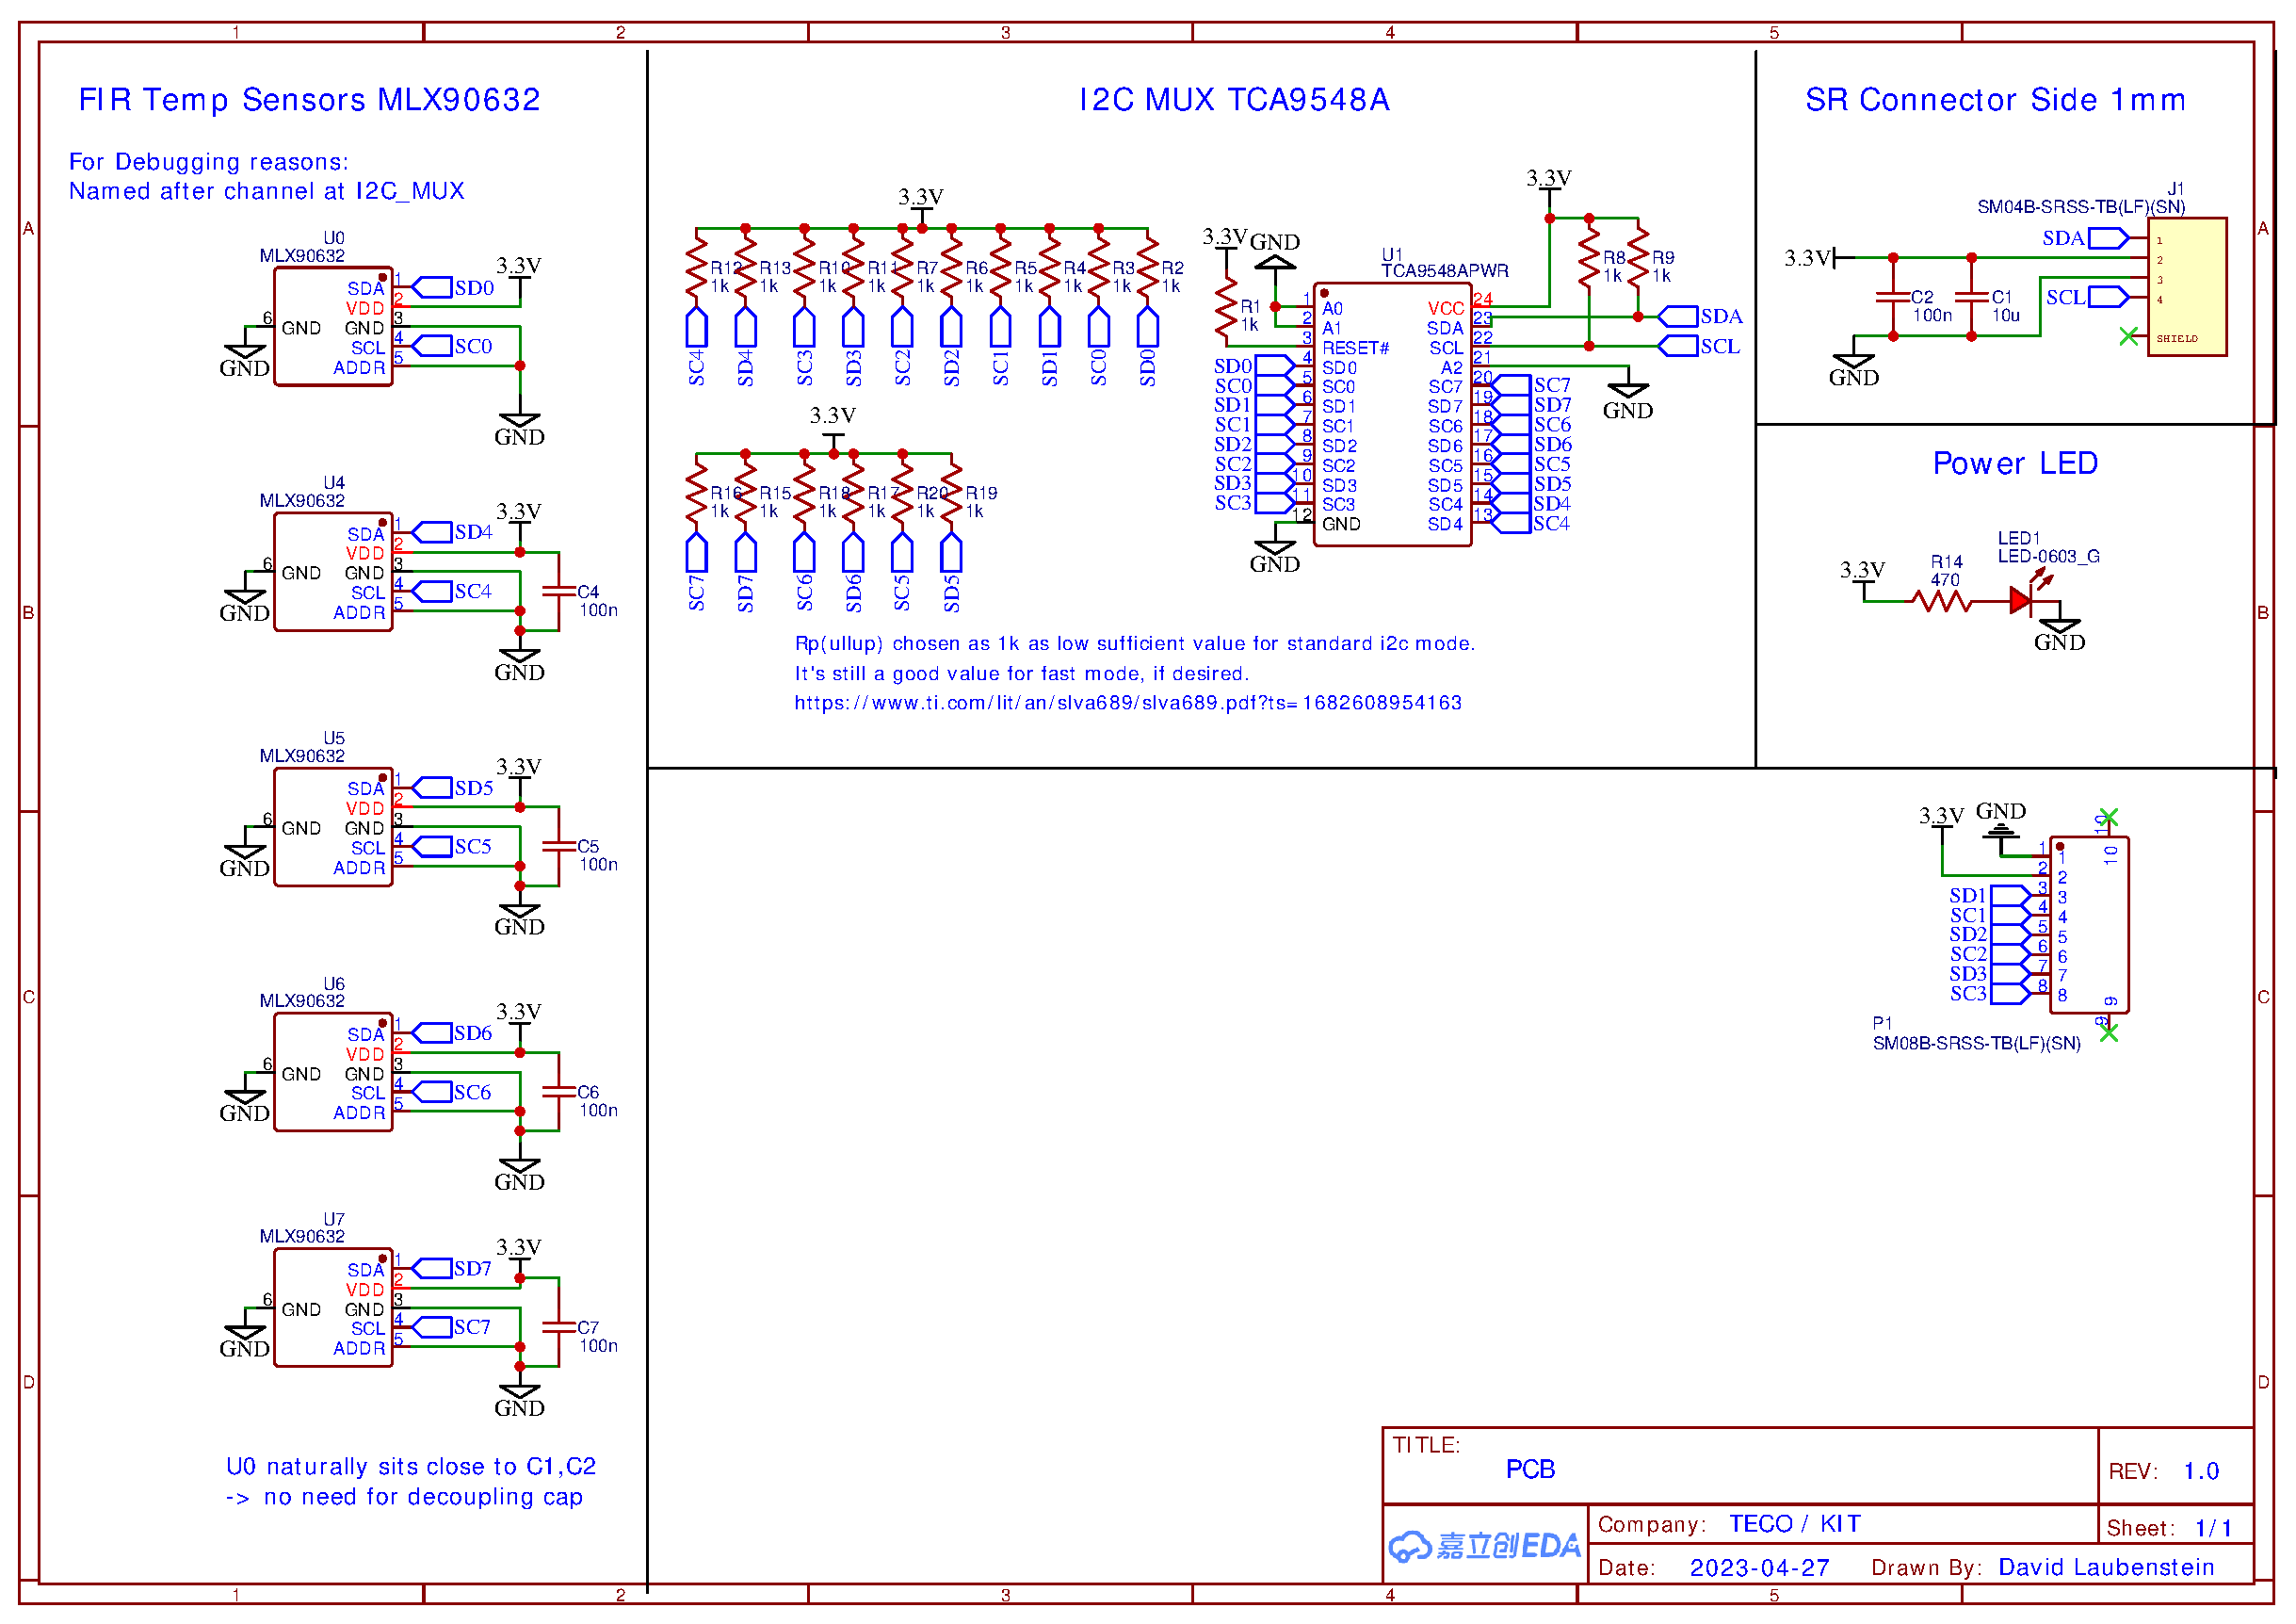
\includegraphics[width=\textwidth]{thesis-doc/images/prototype/schematic/Schematic_Open Earable 1.3 - I2C PCB David_2023-10-17.pdf}
    \caption{Schematic of the PCB which is placed behind the ear.}    
    \label{fig:appendix:schematic_pcb}
\end{figure} 

\begin{figure}
    \centering
    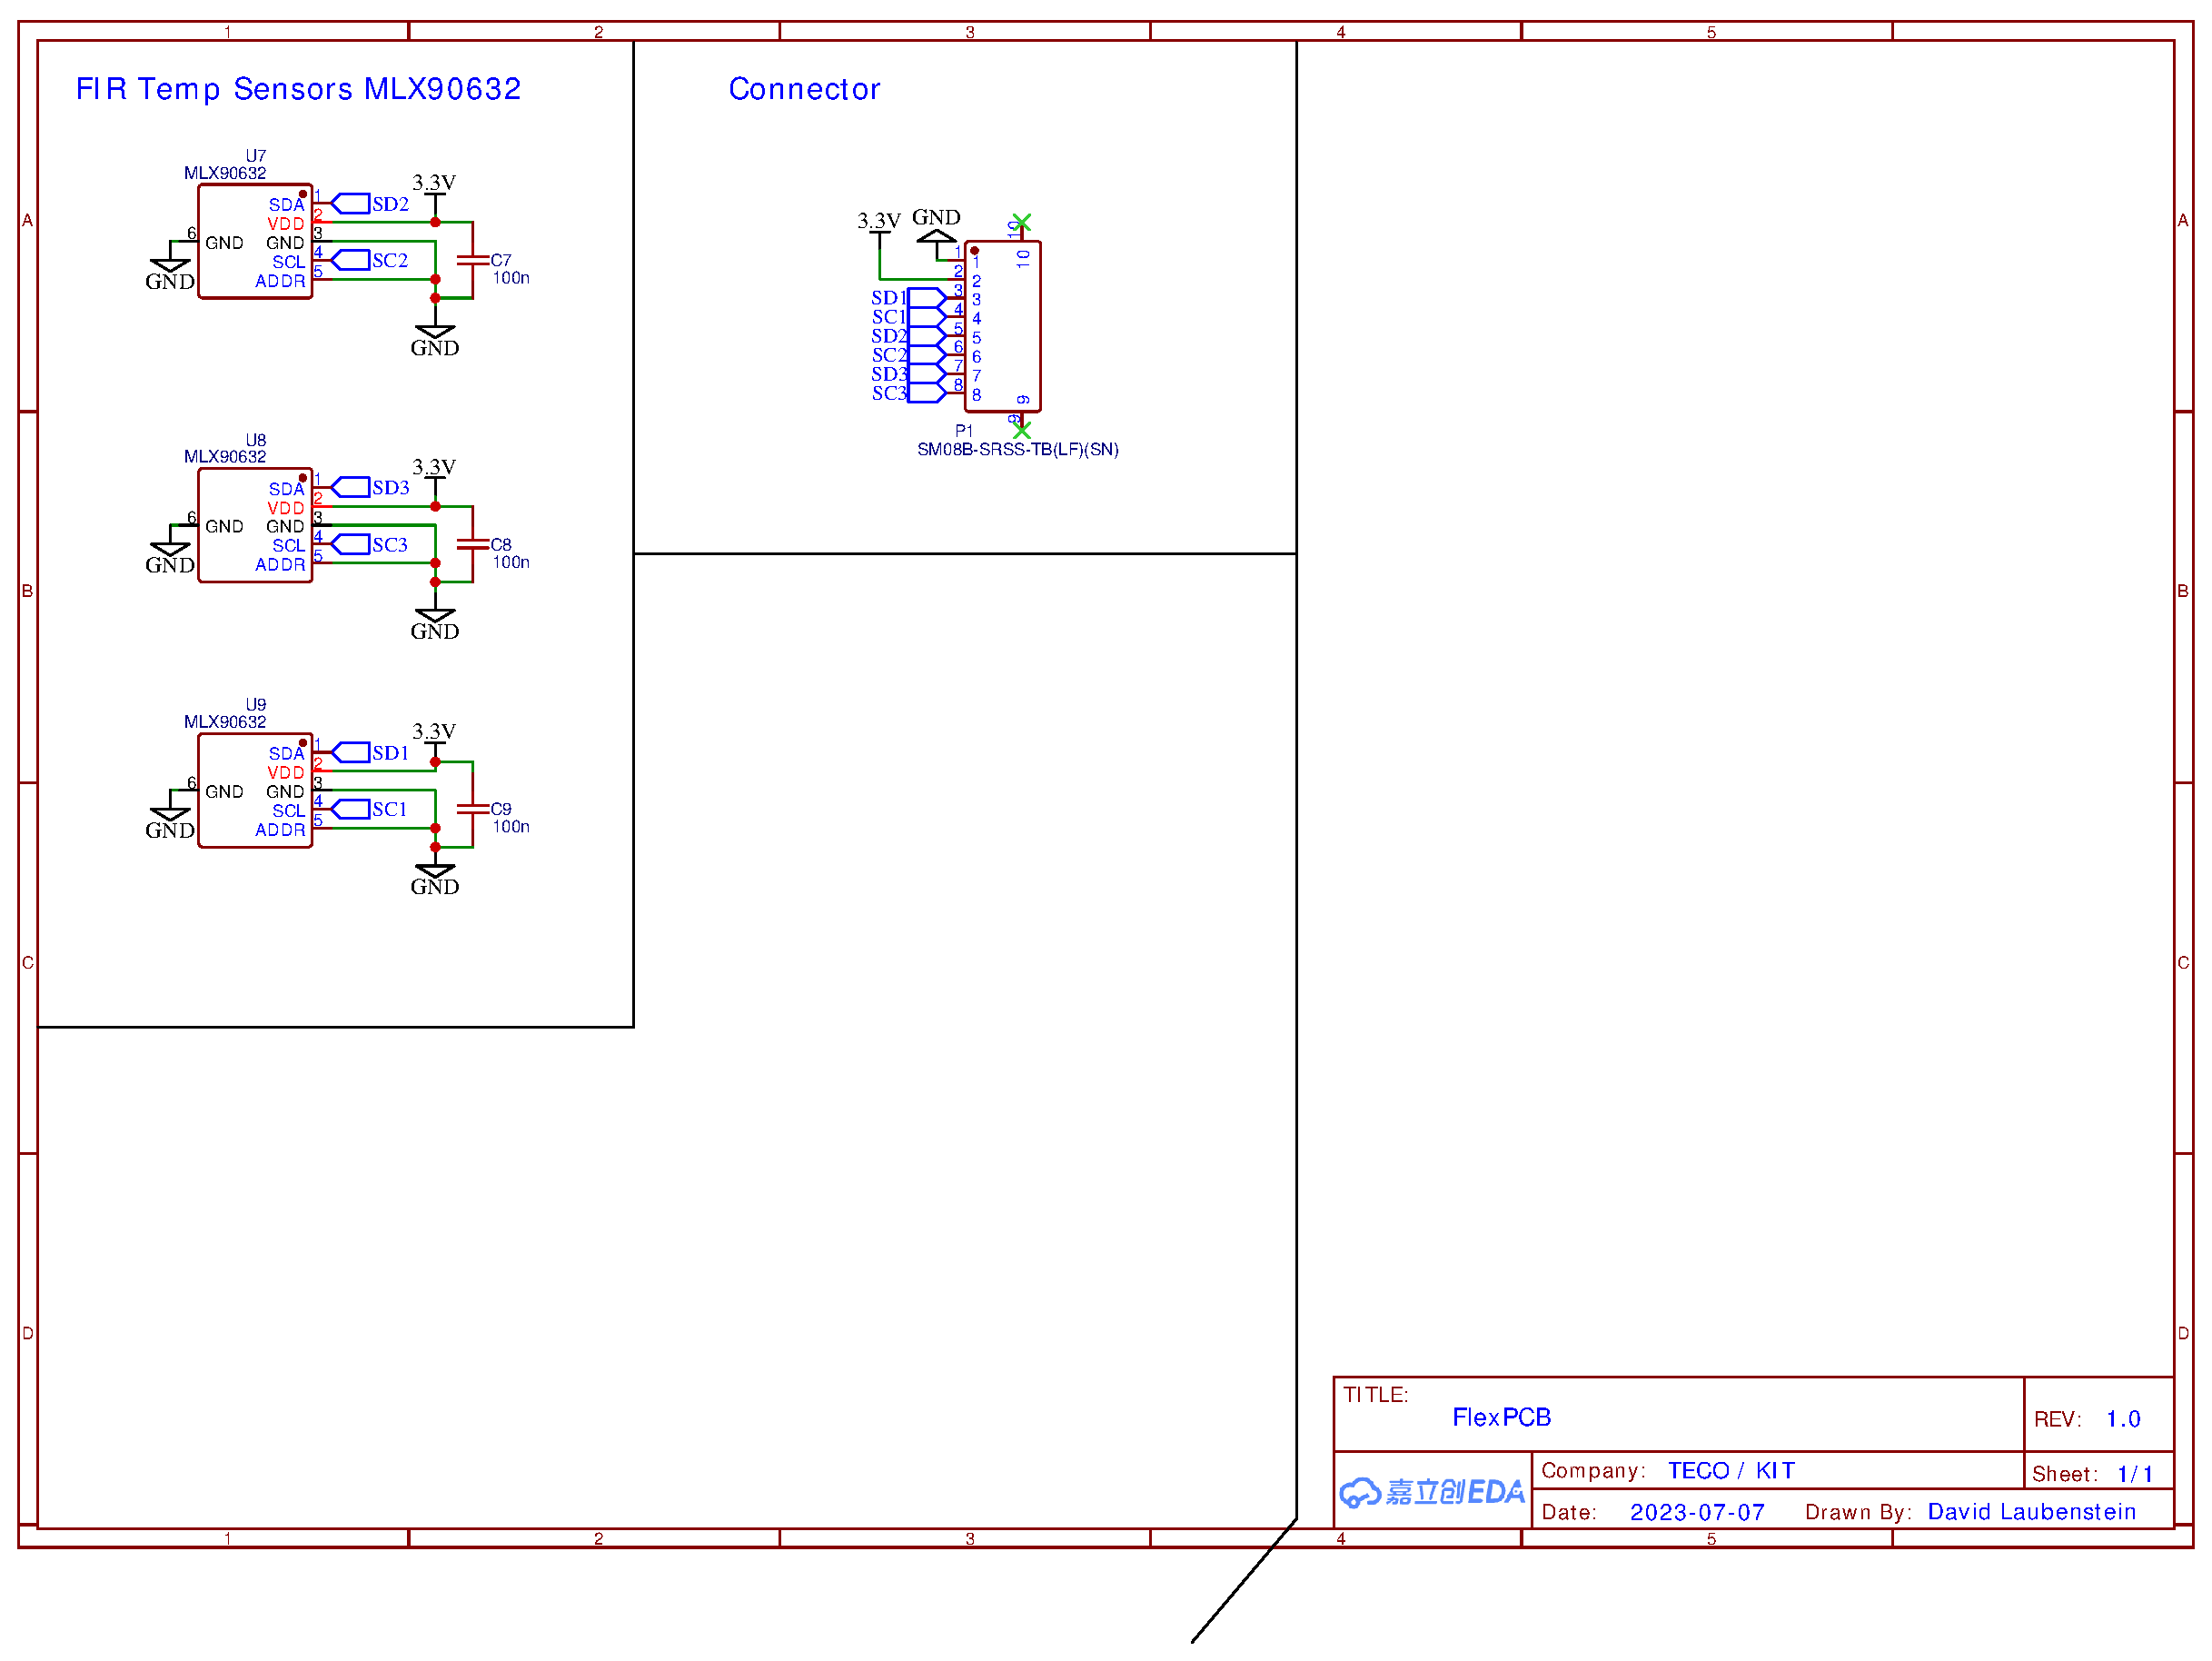
\includegraphics[width=\textwidth]{thesis-doc/images/prototype/schematic/Schematic_Open Earable 1.3 - I2C FlexPCB David_2023-10-17.pdf}
    \caption{Schematic of the FlexPCB which is placed in the prototype in the ear.}    
    \label{fig:appendix:schematic_pcb}
\end{figure} 